\documentclass{standalone}
\usepackage{tikz}
\usetikzlibrary{calc}

% Configuration parameters - EASY TO CHANGE!
\def\startYear{1979}
\def\endYear{1996} 
\def\unitsPerYear{2}
\def\timeStep{3}  % Step between year markers (1=every year, 2=every 2 years, 3=every 3 years, etc.)

% Define a function to convert years to coordinates
\newcommand{\yearToCoord}[1]{%
  \pgfmathparse{(#1-1979)*2-13}%
  \pgfmathresult%
}

% Short version: x{year} returns the x-coordinate using expandable calc syntax
% Centers the timeline so x=0 is at the middle of the timeline
\newcommand{\x}[1]{(#1-\startYear)*\unitsPerYear - (\endYear-\startYear)*\unitsPerYear/2}

\begin{document}

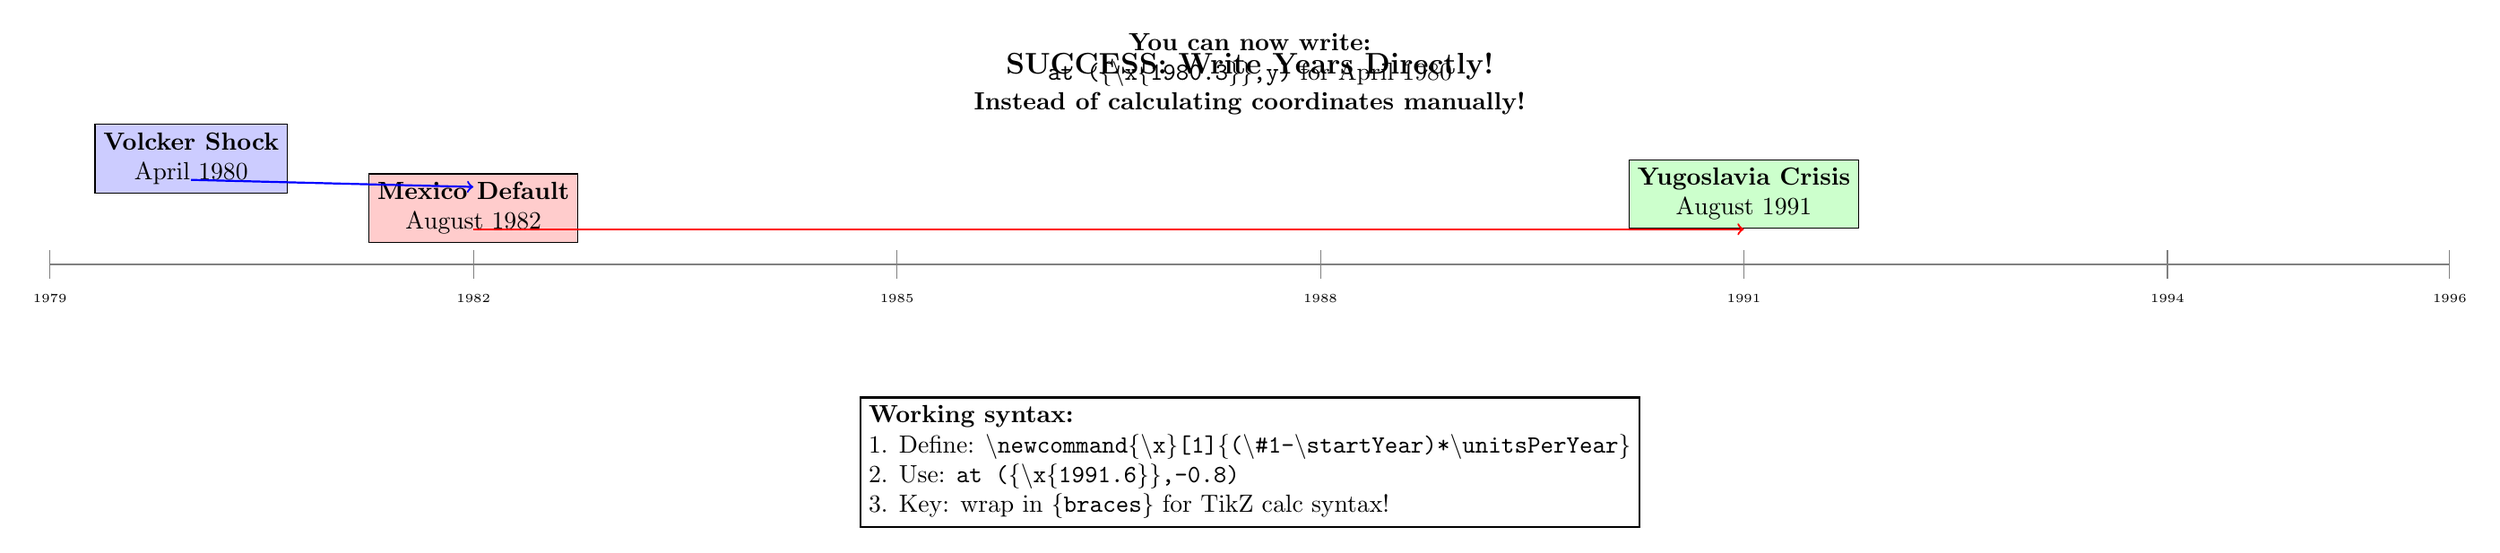
\begin{tikzpicture}

% Calculate timeline bounds dynamically - centered on x=0
\pgfmathsetmacro{\timelineStart}{(\startYear-\startYear)*\unitsPerYear - (\endYear-\startYear)*\unitsPerYear/2}
\pgfmathsetmacro{\timelineEnd}{(\endYear-\startYear)*\unitsPerYear - (\endYear-\startYear)*\unitsPerYear/2}

% Timeline using dynamic coordinates
\draw[gray,thick] (\timelineStart,0) -- (\timelineEnd,0);

% Year markers - automatically generated based on timeStep
\foreach \year in {\startYear,\the\numexpr\startYear+\timeStep\relax,...,\endYear} {
    \draw[gray] ({\x{\year}},-0.2) -- ({\x{\year}},0.2); 
    \node[below,font=\tiny] at ({\x{\year}},-0.3) {\year};
}
% Always include endYear marker if not already covered
\pgfmathtruncatemacro{\lastRegularYear}{\startYear + \timeStep*floor((\endYear-\startYear)/\timeStep)}
\ifnum\lastRegularYear<\endYear
    \draw[gray] ({\x{\endYear}},-0.2) -- ({\x{\endYear}},0.2); 
    \node[below,font=\tiny] at ({\x{\endYear}},-0.3) {\endYear};
\fi

% Events positioned by YEAR
\node[draw,fill=blue!20,align=center] at ({\x{1980}},1.5) {
    \textbf{Volcker Shock}\\April 1980
};

\node[draw,fill=red!20,align=center] at ({\x{1982}},0.8) {
    \textbf{Mexico Default}\\August 1982
}; 

\node[draw,fill=green!20,align=center] at ({\x{1991}},1) {
    \textbf{Yugoslavia Crisis}\\August 1991
};


% Connect events with arrows - now using \x{} command!
\draw[->,thick,blue] ({\x{1980}},1.2) -- ({\x{1982}},1.1);
\draw[->,thick,red] ({\x{1982}},0.5) -- ({\x{1991}},0.5);

% Title showing SUCCESS
\node[above,font=\large\bfseries] at (0,2.5) {SUCCESS: Write Years Directly!};
\node[above,align=center] at (0,2) {
    \textbf{You can now write:} \\
    \texttt{at (\{\textbackslash x\{1980.3\}\},y)} for April 1980 \\
    \textbf{Instead of calculating coordinates manually!}
};

% Show the implementation
\node[draw,thick,align=left] at (0,-2.8) {
    \textbf{Working syntax:}\\
    1. Define: \texttt{\textbackslash newcommand\{\textbackslash x\}[1]\{(\textbackslash\#1-\textbackslash startYear)*\textbackslash unitsPerYear\}}\\
    2. Use: \texttt{at (\{\textbackslash x\{1991.6\}\},-0.8)} \\
    3. Key: wrap in \texttt{\{braces\}} for TikZ calc syntax!
};

\end{tikzpicture}
\end{document}
